%!TEX root = ../../Main.tex
\graphicspath{{Chapters/SystemArkitektur/}}
%-------------------------------------------------------------------------------

\section{System Arkitektur}

Systemarkitekturen i projektet har været en iterativ proces og er derfor blevet rekonstrueret og ændret undervejs i projekt-forløbet.
Arkitekturen i systemet danner rammer for, hvordan BA-TA's logiske system er opbygget og implementeret. Hermed dannes der et overblik over den logiske funktionalitet og hvordan den bruges på tværs af de forskellige drivere i systemet.

\subsection{Entity Relationship Diagram}
På nedenstående figur, \ref{fig:Entity}, danner der et overblik over den logiske funktionalitet på tværs af systemet, som er udmundet i funktioner i de forskellige driver-klasser.

\begin{figure}[H]
	\centering
	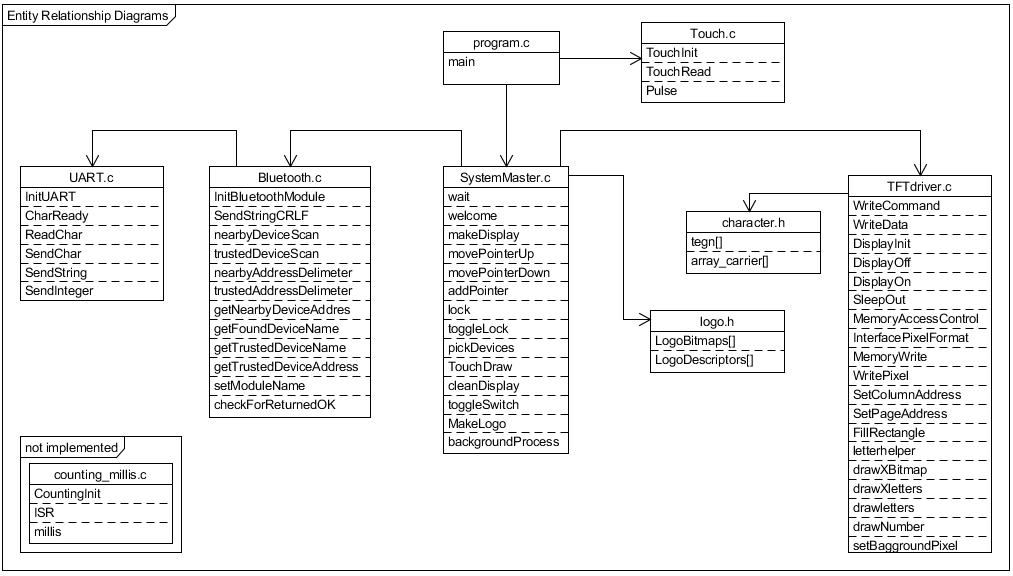
\includegraphics[width = 300 pt]{Img/Entity.png}
	\caption{Entity Relationship Diagrams}
	\label{fig:Entity}
\end{figure}

\subsection{Sekvensdiagrammer}
På nedenstående figur, \ref{fig:Entity}, danner der et overblik over den logiske funktionalitet på tværs af systemet, som er udmundet i funktioner i de forskellige driver-klasser.

\begin{figure}[H]
	\centering
	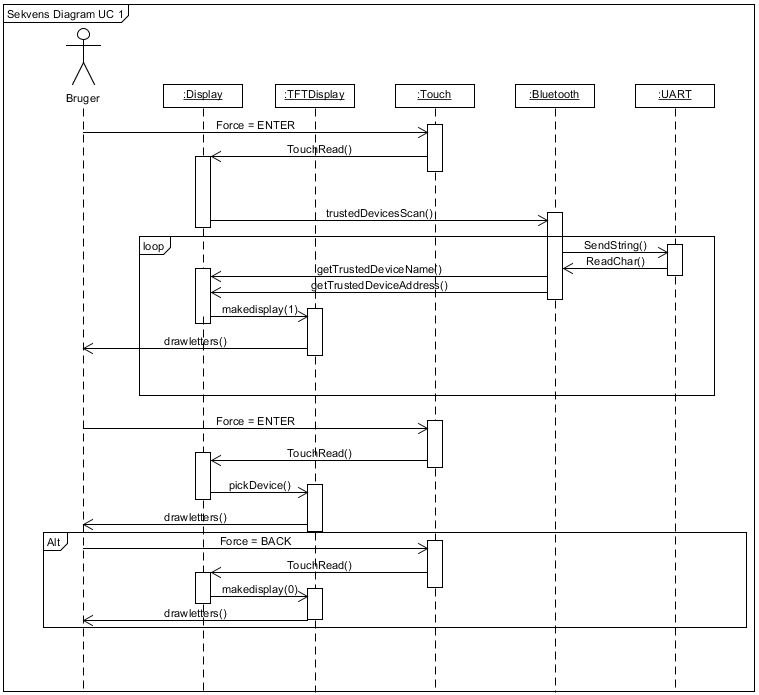
\includegraphics[width = 400 pt]{Img/SD1.png}
	\caption{Sekvensdiagram for use case 1}
	\label{fig:SD1}
\end{figure}

\begin{figure}[H]
	\centering
	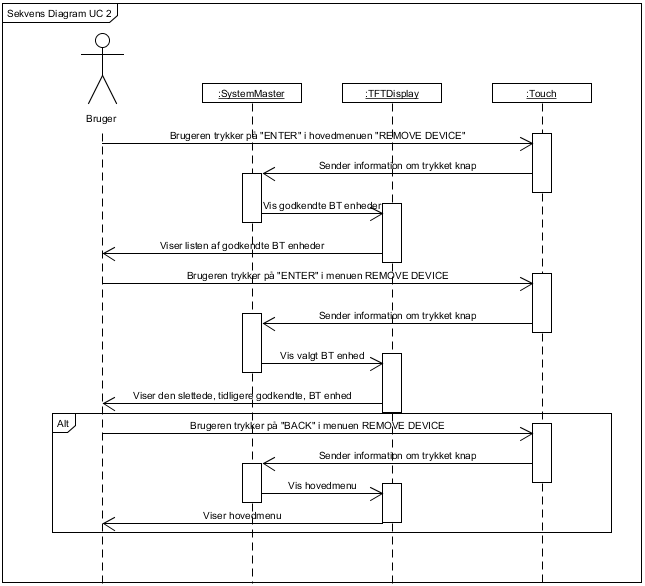
\includegraphics[width = 400 pt]{Img/SD2.png}
	\caption{Sekvensdiagram for use case 2}
	\label{fig:SD2}
\end{figure}

\begin{figure}[H]
	\centering
	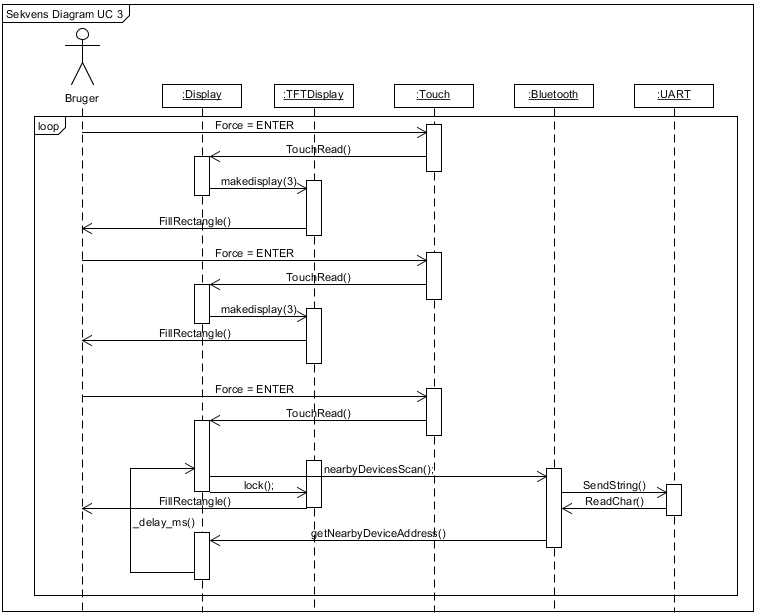
\includegraphics[width = 400 pt]{Img/SD3.png}
	\caption{Sekvensdiagram for use case 3}
	\label{fig:SD3}
\end{figure}